\documentclass[12pt]{article}
\usepackage[utf8]{inputenc}
\usepackage{polski}
\usepackage{hyperref}
\usepackage{listings}
\usepackage{mathtools}
\usepackage{graphicx}
\usepackage{fullpage}
\usepackage{enumerate}
\usepackage{float}
\usepackage{caption}
\usepackage{parskip}
\usepackage{subcaption}
\title{Teoria i Inżynieria Ruchu Teleinformatycznego \\ Sprawozdanie z projektu}
\author{Ewelina Kawecka (201420) \\ Michał Smyk (203254) \\ Mateusz Sitarczyk (203383) \\ Piotr Sobierski (203380)} 
\graphicspath{ {gfx/} }
\begin{document}
\maketitle
\thispagestyle{empty}
\clearpage
\setcounter{page}{1}

\section{Wstęp}
Celem całości projektu było stworzenie programu, który na podstawie historii ruchu w sieci komputerowej będzie w stanie przeanalizować go pod kątem interesujących właściwości, które mogą być w tej historii zawarte. Projekt podzielony został na dwie części. Pierwsza część projektu jest odpowiedzialna za ekstrakcję danych z plików PCAP, zawierających nagrane informacje na temat historii ruchu w sieci. Druga część projektu ma za zadanie na podstawie otrzymanych danych wyekstraktować kod html a następnie przetworzyć go pod kątem częstotliwości występowania elementów takich jak: rozszerzenia obrazków, klasy html, tagi html, rodzaje linków. Dodatkowym zadaniem proponowanej aplikacji jest wydobywanie z otrzymywanych danych obrazków i zapis ich w pamięci. 

\section{Opis problemu}
Głównym problemem, na którym skupia się pierwsza część projektu jest ekstrakcja i filtrowanie danych zawartych w pliku PCAP. Z racji, że w plikach tych znajdują się również dodatkowe informacje, które ze względu na brak przydatności do celów zadania powinny zostać odfiltrowane. Pozostałe dane, które przechowują przydatne informacje powinny zostać przetworzone w taki sposób, aby umożliwić odczytanie z nich informacji, które interesują osobę wykorzystującą program. Filtracja i ekstrakcja danych podzielona została na kilka etapów, które w postaci funkcji udostępniane są przez program. Funkcje te przedstawia rysunek \ref{img:funkcje}.

\begin{figure}[h]
\centering
\caption{Atomowe usługi opracowane w ramach pierwszej części projektu}
\label{img:funkcje}
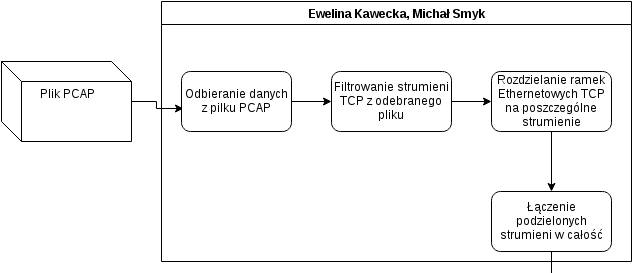
\includegraphics[width=0.7\textwidth]{Wykres.png}
\end{figure}


Odfiltrowane i przetworzone dane muszą zostać następnie poddane kolejnemu procesowi, którego zadaniem jest wydobycie kodu html w czystej postaci. Podczas ekstrakcji html należy również zwrócić uwagę na kompresję danych i w przypadku jej wystąpienia konieczne jest odpowiednia dekompresja kodu. 
Tak przygotowane dane poddawane są później m.in. analizie statystycznej (Rysunek \ref{img:funkcje2}). 

\begin{figure}[h]
\centering
\caption{Atomowe usługi opracowane w ramach drugiej części projektu}
\label{img:funkcje2}
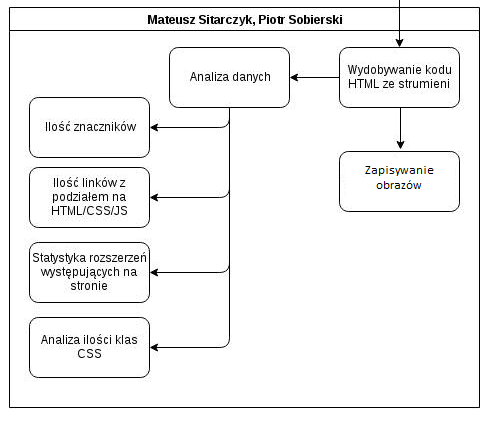
\includegraphics[width=0.7\textwidth]{Wykres2.png}
\end{figure}


Zgodnie z zaleceniami prowadzącego każda atomowa funkcja realizowana przez program udostępniona jest w formie usługi - szczegółowe informacje na ich temat dostępne są w rozdziale \ref{dzialanie}. 

\section{Opis implementacji programu}
\label{dzialanie}
\subsection{Ekstrakcja danych}
Wstępnie otrzymane z pliku PCAP zapisy historii połączeń zostają w pierwszym etapie przeczyszczone za pomocą biblioteki \emph{dpkt}. Aplikacja łączy się z pierwszą z usług, w celu wyodrębnienia tych danych, które zawierają paczki Ethernetowe. Następnie paczki te przesyłane są do kolejnej usługi, która zajmuje się podzieleniem ich na podstawie zawartości - grupując poszczególne paczki za pomocą krotek (\emph{IP nadawcy}, \emph{port nadawcy}, \emph{IP odbiorcy}, \emph{Port odbiorcy}). Pogrupowane w ten sposób strumienie łączone są w jeden spójny poprzez kolejną usługę.
\subsection{Ekstrakcja HTML}
Tak spreparowane dane przesyłane są następnie do pliku html\_extractor.py, w którym odbywa się wydobywanie kodu html. 
Ponieważ aplikacja ma za zadanie analizować ruch internetowy należy brać pod uwagę tylko dane przesyłana na porcie 80. Ze względu na fakt, że interesują nas tylko odpowiedzi serwera omawiany moduł ignoruje treść samych zapytań. Odczytanie danych jest możliwe dzięki wykorzystaniu biblioteki dpkt. Dekompresja danych odbywa się przy pomocy biblioteki gzpi po uprzednim sprawdzeniu zawartości nagłówka 'content-encoding'. Zadaniem modułu jest również ekstrakcja obrazków. Osiągane jest to poprzez weryfikacje nagłówka 'content-type', jeśli nagłówek ten zawiera wartości typowe dla obrazów to aplikacja zapisuje otrzymany obraz w dedykowanym folderze. Ostatecznie moduł przesyła dane dalej do pliku html\_receiver.py, którego zadaniem jest właściwie tylko dalsze przekazanie kodu do usług odpowiedzialnych za analizę statystyczną.

\subsection{Analiza HTML}
Analiza każdej z zaimplementowanych właściwości kodu HTML jest realizowana przez dwa oddzielne pliki: plik serwera - zajmujący się odbieraniem danych oraz plik analizujący - odpowiedzialny za samo przetwarzanie danych. Wszystkie pliki serwerowe, podobnie jak miało to miejsce w opisanych wcześniej modułach oparte są na bibliotece socket. Odbierają one kod html a następnie wywołują odpowiednie metody analizujące dane. Każdy z modułów analizujących wykorzystuje bibliotekę HTMLParser. W nich zaimplementowane są klasy dziedziczące po HTMLParser i nadpisujące metodę handle\_starttag. To właśnie w niej odbywa się cała analiza kodu. Dla każdej instancji tej klasy tworzona jest również tablica asocjacyjna w której przechowywane są wyniki analizy w poszczególnych krokach. Cechą wspólną modułów jest też fakt, że na podstawie otrzymanych danych z wykorzystaniem biblioteki matplotlib.pyplot zapisywane są wykresy reprezentujące wyniki.\\
Pierwszy z modułów znajduje się w pliku images\_analyzer.py, a zadaniem jego jest wyodrębnienie ile obrazków, z podziałem na rozszerzenia, znajduje się na stronie. Analizowany jest tak img a następnie jego atrybut src.\\
Drugi moduł odpowiedzialny jest za analizę ile razy poszczególne klasy css zostały wykorzystane w kodzie strony. Moduł ten zaimplementowany jest w pliku css\_class\_analyzer.py. Dla każdego znacznika sprawdzany jest jego atrybut class i zliczane są wszystkie wystąpienia klas w nim się znajdujących.\\
Następnym moduł odpowiedzialny jest za zliczanie liczności wykorzystanych tagów. Algorytm zaimplementowany jest w pliku tag\_sanalyzer.py i opiera się na zliczania kolejnych rozpoczynających się tagów w otrzymanym kodzie.\\
Ostatni moduł znajduje się w pliku links\_analyzer.py. Zlicza on ilość linków zewnętrznych oraz wewnętrznych, liczbę plików JavaScript'owych wewnętrznych, zewnętrznych oraz znajdujących się bezpośrednio w kodzie i na podobnej zasadzie pliki css. W przypadku linków analizowany jest tag a i jest atrybut href, przy plikach js tag script i ewentualny atrybut src, natomiast przy plikach css tag link, jego atrybut rel oraz ewentualny atrybut href.

\section{Opis usług}
\subsection{DataExtraction/sender.py}
Usługa odpowiadająca za załadowanie z pliku PCAP danych. Jako pierwszy argument przyjmuje nazwę pliku PCAP. 
\mbox{}\\\\
\textbf{Komunikuje się z usługami:}\\
\begin{itemize}
\item DataExtraction/receiver.py
\end{itemize} 

\subsection{DataExtraction/receiver.py}
Usługa odpowiadająca za odebranie załadowanych danych do dalszego przetwarzania. Za pomocą Socketu nasłuchuje ona połączenia z plikiem sender.py, agregując odebrane dane w postaci listy i przesyłając je do dalszego przetwarzania.
\mbox{}\\\\
\textbf{Komunikuje się z usługami:}\\
\begin{itemize}
\item DataExtraction/sender.py
\end{itemize} 

\subsection{DataExtraction/frame\_filter.py}
Usługa odpowiadająca za filtrowanie ramek, które nie pochodzą z pakietów typu Ethernet.

Usługa ta nie wymaga współpracy z żadną z innych usług - przyjmuje dane załadowane z pliku PCAP, a następnie zwraca te same dane, z wyłączeniem tych, które powinny być odrzucone. 

\subsection{DataExtraction/merger.py}
Usługa odpowiadająca za grupowanie ramek, które zostały przefiltrowane przez poprzednią usługę. Usługa ta zarówno grupuje, jak i łączy strumienie w spójne dane, przesyłane do dalszych usług.

\subsubsection{DataExtraction/html\_extractor.py} 
Usługa odpowiedzialna za wydobywanie kodu html i obrazów.
\mbox{}\\\\
\textbf{Komunikuje się z usługami:}\\
\begin{itemize}
\item DataAnalysys/html\_receiver.py
\end{itemize} 

\subsubsection{DataAnalysys/html\_receiver.py} 
Usługa odpowiedzialna za przekazywanie html do pozostałych usług analizujących dane.
\mbox{}\\\\
\textbf{Komunikuje się z usługami:}\\
\begin{itemize}
\item DataAnalysys/css\_class\_server.py
\item DataAnalysys/images\_server.py
\item DataAnalysys/links\_server.py
\item DataAnalysys/tags\_server.py
\end{itemize} 

\subsubsection{DataAnalysys/css\_class\_server.py} 
Usługa odpowiedzialna za generowanie statystyk dotyczących częstotliwości występowania poszczególnych klas css.

\subsubsection{DataAnalysys/images\_server.py} 
Usługa odpowiedzialna za generowanie statystyk dotyczących częstotliwości występowania obrazów o poszczególnych rozszerzeniach.

\subsubsection{DataAnalysys/links\_server.py} 
Usługa odpowiedzialna za generowanie statystyk dotyczących częstotliwości występowania różnych typów linków.

\subsubsection{DataAnalysys/tags\_server.py} 
Usługa odpowiedzialna za generowanie statystyk dotyczących częstotliwości występowania poszczególnych typów znaczników html.


\section{Przykładowe wywołanie}
\subsection{Sposób wywołania}
Program wywołujemy poprzez uruchomienie wszystkich usług, które składają się na jego elementy:
\begin{itemize}
\item DataExtraction/main.py (Uruchomienie usługi filtrującej dane z pliku pcap)
\item DataAnalysys/main.py (Uruchomienie usługi odbierającej kod html)
\item DataAnalysys/main1.py (Uruchomienie usługi analizującej obrazy)
\item DataAnalysys/main2.py (Uruchomienie usługi analizującej klasy css)
\item DataAnalysys/main3.py (Uruchomienie usługi analizującej tagi html)
\item DataAnalysys/main4.py (Uruchomienie usługi analizującej linki)
\end{itemize}

Po uruchomieniu powyższych usług należy przy pomocy pliku \emph{DataExtraction/sender.py} przesłać dane z pliku \emph{.pcap}, co rozpocznie dalsze przetwarzanie i proces analizy. 

\subsection{Przykładowe wyniki}
W celu przeprowadzenia testów utworzony został przykładowy plik \emph{.pcap}, który nagrany został podczas przeglądania stron internetowych takich jak: \emph{wp.pl}, \emph{wykop.pl} oraz \emph{onet.pl}. 

W wyniku działania programu wygenerowane zostały następujące wykresy:

\begin{figure}[h]
\centering
\caption{Przykładowy wykres dla częstości występowania klas css.}
\label{img:wykresCss}
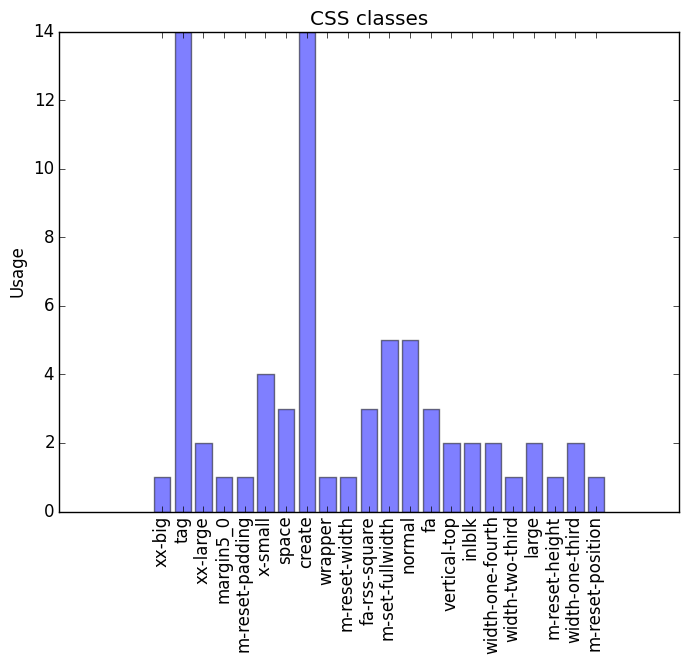
\includegraphics[width=0.7\textwidth]{WykresCss.png}
\end{figure}

\begin{figure}[h]
\centering
\caption{Przykładowy wykres dla częstości występowania tagów html.}
\label{img:wykresTagi}
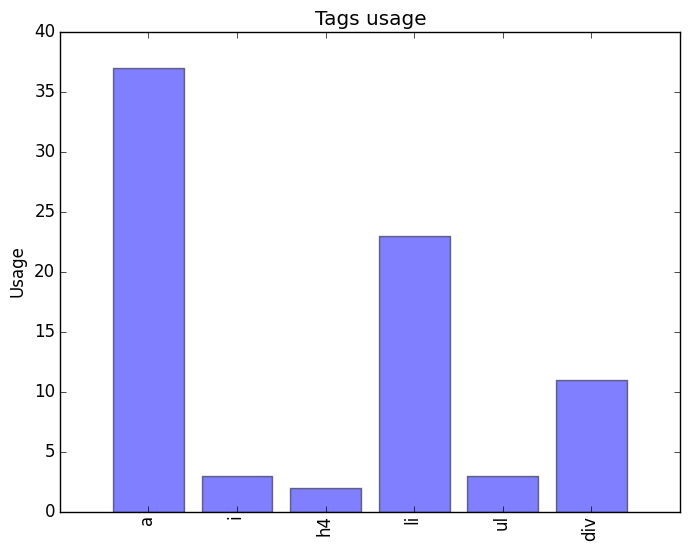
\includegraphics[width=0.7\textwidth]{WykresTagi.png}
\end{figure}

\begin{figure}[h]
\centering
\caption{Przykładowy wykres dla częstości występowania obrazków o poszczególnych rozszerzeniach.}
\label{img:wykresObrazki}
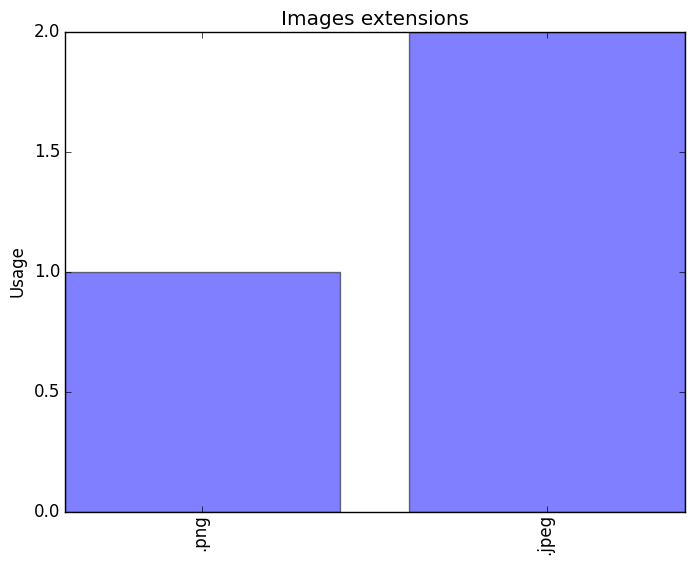
\includegraphics[width=0.7\textwidth]{WykresObrazki.png}
\end{figure}

\begin{figure}[h]
\centering
\caption{Przykładowy wykres dla częstości występowania różnych typów linków.}
\label{img:wykresLinków}
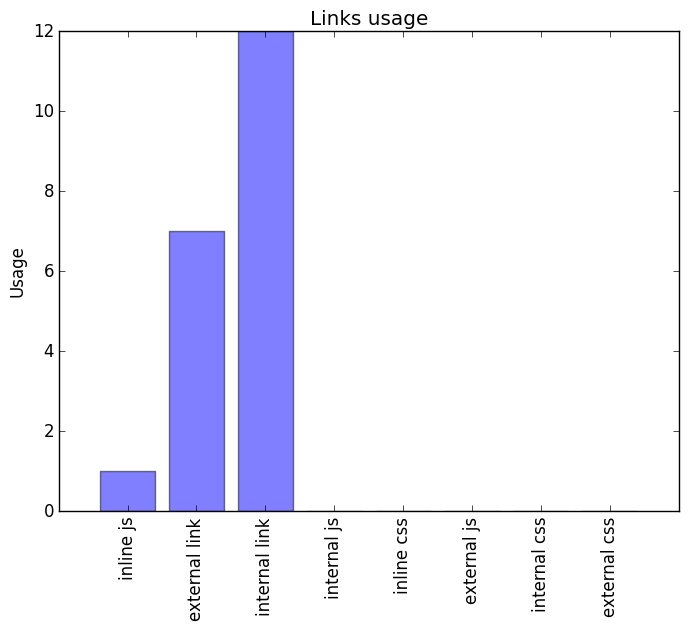
\includegraphics[width=0.7\textwidth]{WykresLinki.png}
\end{figure}


\end{document}
